\documentclass[paper=a4, fontsize=11pt, onecolumn, tikz, dvipsnames, svgnames, x11names]{article}
\usepackage[utf8]{inputenc}
\usepackage[T1]{fontenc}
\usepackage[english]{babel}
\usepackage{multicol}
\usepackage{fullpage}
% ------------------------- Color table ----------------------------------------
\usepackage{multirow}
\usepackage[table]{xcolor}
\definecolor{maroon}{cmyk}{0,0.87,0.68,0.32}
\usepackage{booktabs} % to make prettier tables (toprule, midrule, bottomrule)
% ------------------------------------------------------------------------------

\usepackage{amscd}
\usepackage{amsthm}
\usepackage{physics}
\usepackage{textcomp,gensymb} %pour le °C, et textcomp pour éviter les warning
\usepackage{graphicx} %pour les images
\usepackage{caption}
\usepackage{subcaption}
\usepackage[colorlinks=true,
	breaklinks=true,
	citecolor=blue,
	linkcolor=blue,
	urlcolor=blue]{hyperref} % pour insérer des liens
\usepackage{epstopdf} %converting to PDF
\usepackage[export]{adjustbox} %for large figures

\usepackage{array}
\usepackage{dsfont}% indicatrice : \mathds{1}


% -------------------------- Mathematics ---------------------------------------
\graphicspath{{images/}{../images/}} % For the images path
% ------------------------------------------------------------------------------

% -------------------------- Mathematics ---------------------------------------
\usepackage{mathrsfs, amsmath, amsfonts, amssymb}
\usepackage{bm}
\usepackage{mathtools}
\usepackage[Symbol]{upgreek} % For pi \uppi different from /pi
\newcommand{\R}{\mathbb{R}} % For Real space
\usepackage{tikz}
\usetikzlibrary{bayesnet} %library to draw graphical models1
% ------------------------------------------------------------------------------


% -------------------------- Code format ---------------------------------------
\usepackage[numbered,framed]{matlab-prettifier}
\lstset{
	style              = Matlab-editor,
	basicstyle         = \mlttfamily,
	escapechar         = '',
	mlshowsectionrules = true,
}
% ------------------------------------------------------------------------------

% ------------------------- Blbiographie --------------------------------------
% \usepackage[backend=biber, style=ieee]{biblatex}
% \addbibresource{biblio.bib}
% \bibliography{../material/biblio.bib}
% \usepackage{csquotes}
% ------------------------------------------------------------------------------


\setcounter{tocdepth}{4} %Count paragraph
\setcounter{secnumdepth}{4} %Count paragraph
\usepackage{float}

\usepackage{graphicx} % for graphicspath
% \graphicspath{{../images/}}

\usepackage{array,tabularx}
\newcolumntype{L}[1]{>{\raggedright\let\newline\\\arraybackslash\hspace{0pt}}m{#1}}
\newcolumntype{C}[1]{>{\centering\let\newline\\\arraybackslash\hspace{0pt}}m{#1}}
\newcolumntype{R}[1]{>{\raggedleft\let\newline\\\arraybackslash\hspace{0pt}}m{#1}}


% \usepackage{algpseudocode}
% \usepackage{algorithm}
\usepackage{hyperref}
\usepackage[edges]{forest}

% ------------------------------ Jules packages --------------------------------
\usepackage[ruled,vlined]{algorithm2e}
\usepackage[colorinlistoftodos]{todonotes}
\usepackage{alltt}

% Independent sign
\newcommand{\indep}{\ensuremath{\,\bot\!\!\!\bot\,}} %% The symbol for independent

% Alpha / Numbers for sections
\renewcommand{\thesubsubsection}{\arabic{section}.\arabic{subsection}.\alph{subsubsection})}

\newcommand{\argmin}[1]{\underset{#1}{\operatorname{argmin}}\;}

% % Norm
% \newcommand{\norm}[1]{\left\lVert#1\right\rVert}


% ------------------------ General informations --------------------------------
\title{\normalfont \normalsize \huge Pointing error correction}
\author{Jules Kozolinsky, Vincent Matthys}
\graphicspath{{images/}{../images/}} % For the images path
% ------------------------------------------------------------------------------


\date{}

\begin{document}
\maketitle

% \begin{tabularx}{0.9\textwidth}{@{} l X r @{} }
% 	{\textsc{Master MVA}}  &  & \textsc{} \\
% 	\textsc{Remote sensing} &  & {ENS Paris Saclay}       \\
% \end{tabularx}
% \vspace{1.5cm}
% \begin{center}
%
% 	\rule[11pt]{5cm}{0.5pt}
%
% 	\textbf{\LARGE \textsc{Pointing error correction}}
% 	\vspace{0.5cm}
%
% 	Jules Kozolinsky,
% 	Vincent Matthys
%
% 	jules.kozolinsky@ens-cachan.fr\\
% 	vincent.matthys@ens-paris-saclay.fr
%
% 	\rule{5cm}{0.5pt}
%
% 	\vspace{1.5cm}
% \end{center}

\section{Planet data}

\subsection{Structure}


\begin{forest}
  my label/.style={
    label={[font=\sffamily]right:{#1}},
  },
  for tree={
    folder,
    font=\sffamily,
    text=white,
    minimum height=0.75cm,
    if level=0{fill=ForestGreen}{fill/.wrap pgfmath arg={SlateBlue#1}{int(4-(mod((level()-1),4)))}},
    rounded corners=4pt,
    grow'=0,
    edge={ForestGreen,rounded corners,line width=1pt},
    fit=band,
  },
  [data
    [s03\_20161003T161107Z
      [panchromatic
        [s03\_20161003T161107Z\_pan\_d1\_0001\_rpc.txt]
        [s03\_20161003T161107Z\_pan\_d1\_0001.tif]
      ]
      [pansharp
        [s03\_20161003T161107Z\_pansharp\_bgrn\_d1\_0001\_rpc.txt]
        [s03\_20161003T161107Z\_pansharp\_bgrn\_d1\_0001.tif]
      ]
    ]
    [s03\_20161003T161148Z
      [panchromatic
        [s03\_20161003T161148Z\_pan\_d1\_0001\_rpc.txt]
        [s03\_20161003T161148Z\_pan\_d1\_0001.tif]
      ]
      [pansharp
        [s03\_20161003T161148Z\_pansharp\_bgrn\_d1\_0001\_rpc.txt]
        [s03\_20161003T161148Z\_pansharp\_bgrn\_d1\_0001.tif]
      ]
    ]
    [s03\_20161003T161231Z
      [panchromatic
        [s03\_20161003T161231Z\_pan\_d1\_000\_rpc.txt]
        [s03\_20161003T161231Z\_pan\_d1\_0001.tif]
      ]
      [pansharp
        [s03\_20161003T161231Z\_pansharp\_bgrn\_d1\_0001\_rpc.txt]
        [s03\_20161003T161231Z\_pansharp\_bgrn\_d1\_0001.tif]
      ]
    ]
  ]
\end{forest}

\subsection{Geolocalisation}

\newpage
\begin{figure}
    \centering
    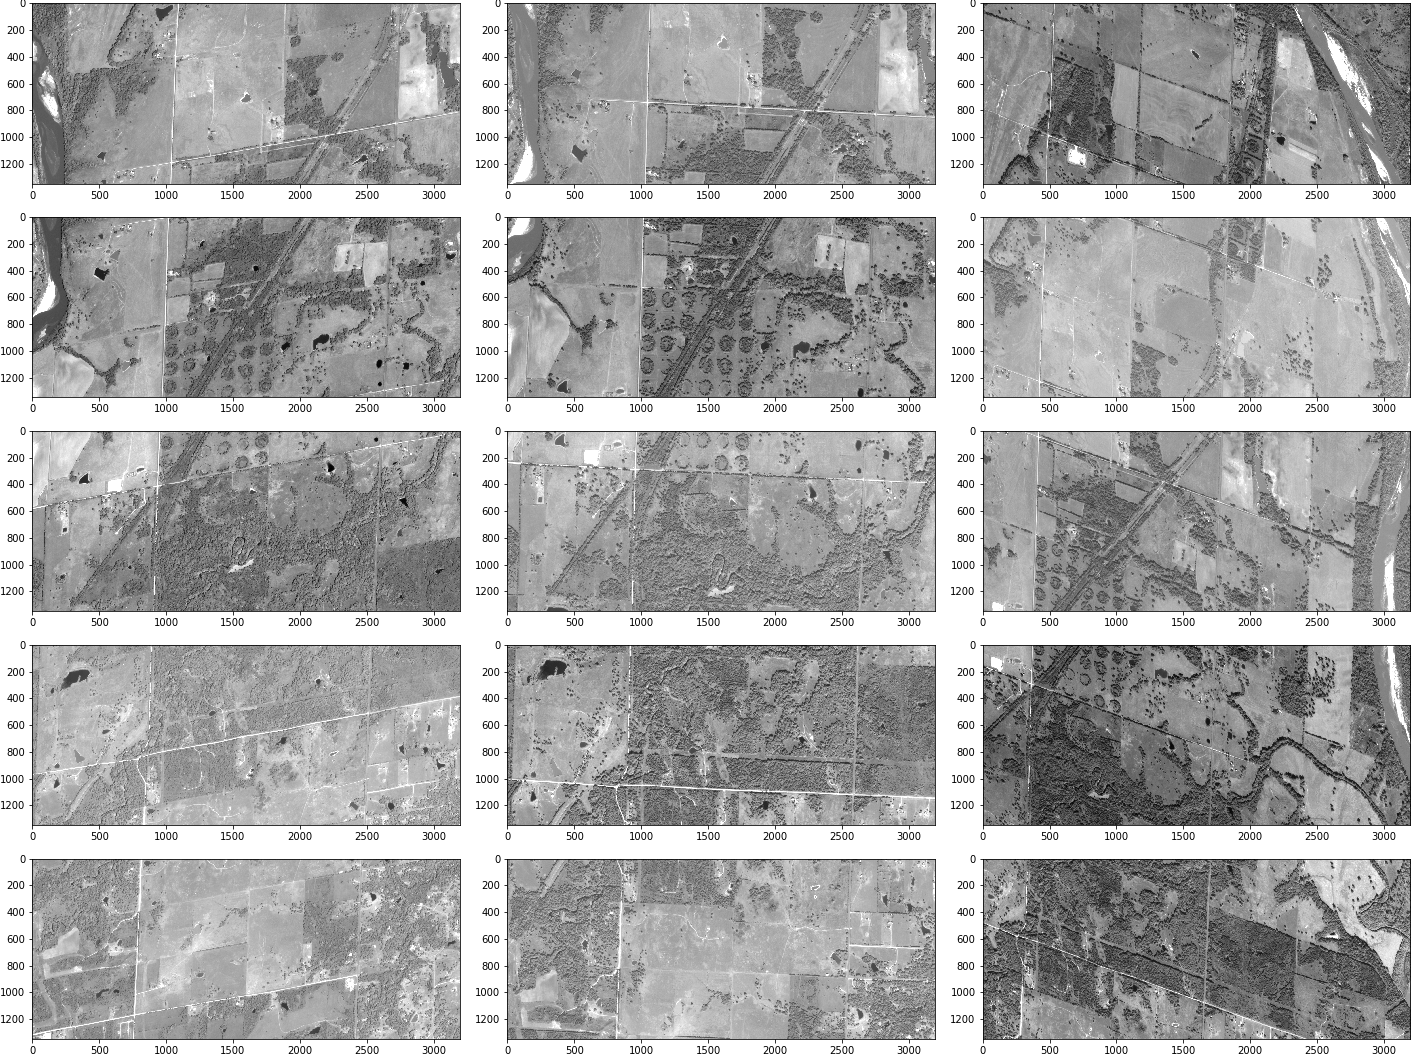
\includegraphics[width = 0.95\textwidth]{d1.png}
    \caption{Mosaic of d1. From left to right: 1Z, 7Z, 8Z}
    \label{}
\end{figure}

\newpage
\begin{figure}
    \centering
    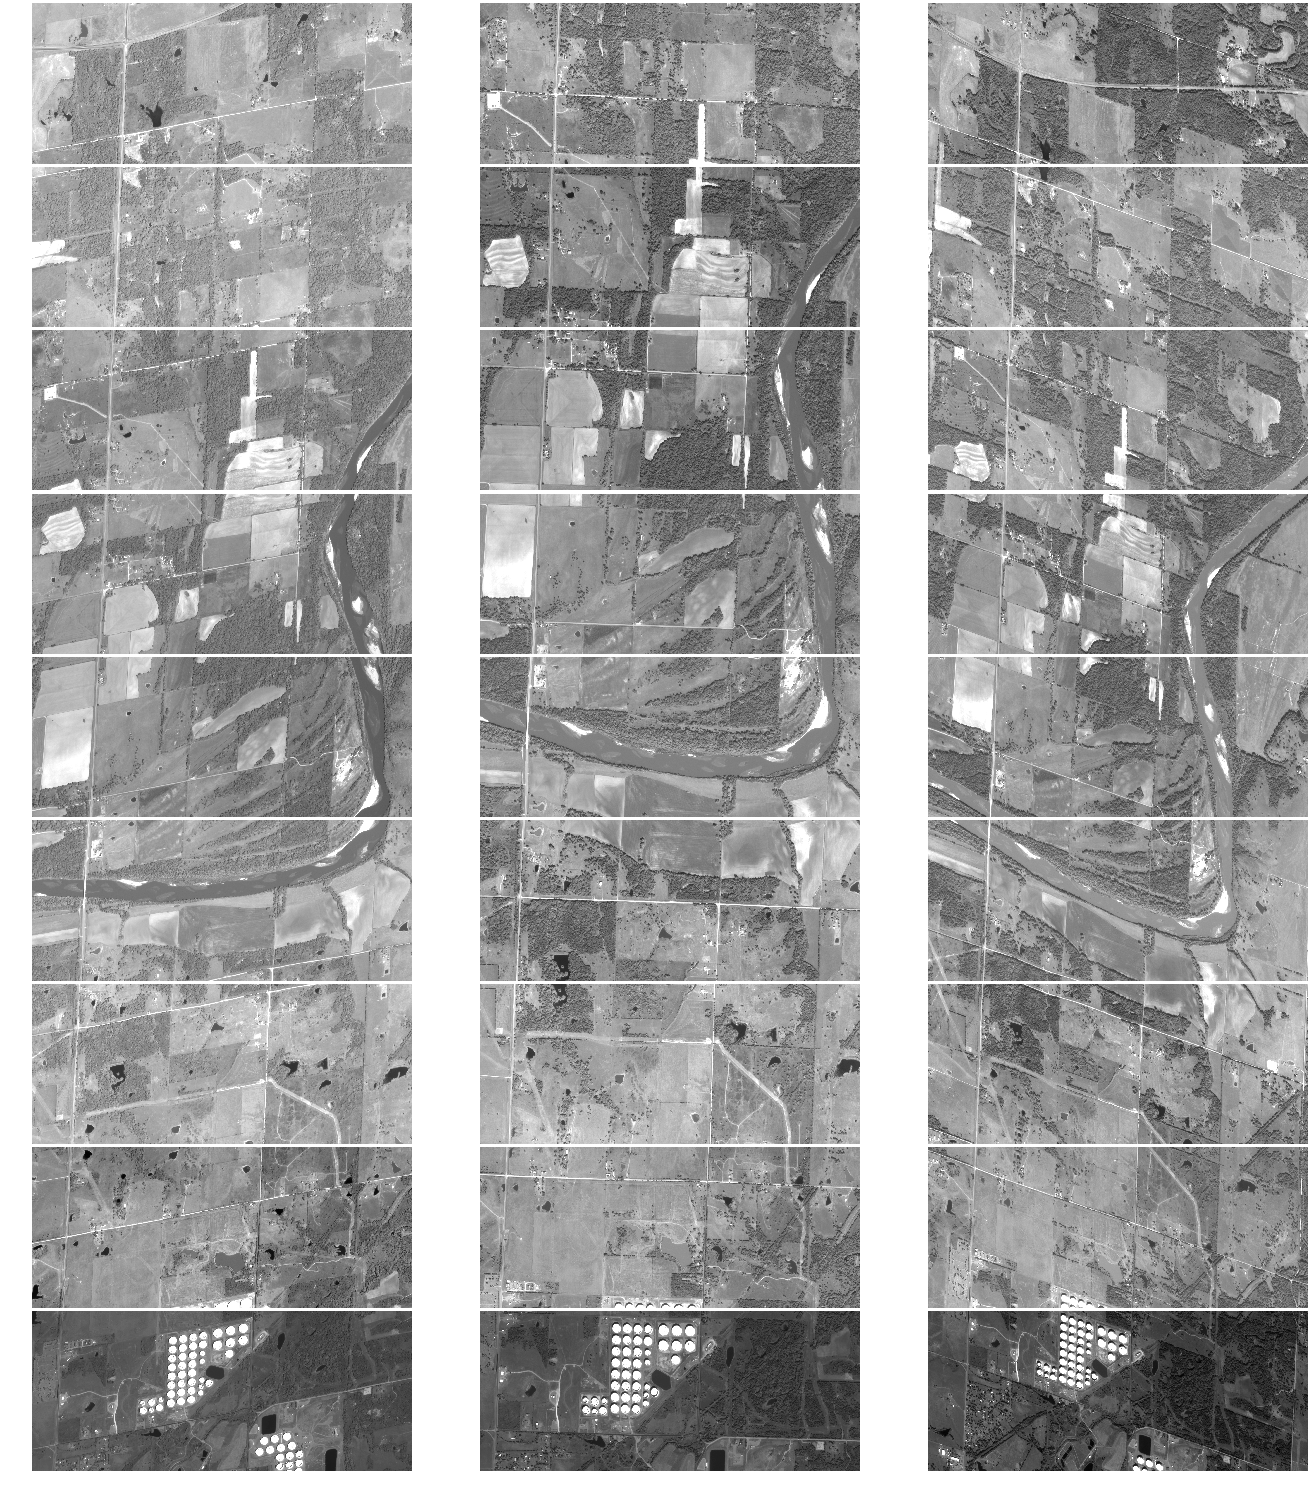
\includegraphics[width = 0.95\textwidth]{d2.png}
    \caption{Mosaic of d2. From left to right: 1Z, 7Z, 8Z}
    \label{}
\end{figure}

\newpage
\begin{figure}
    \centering
    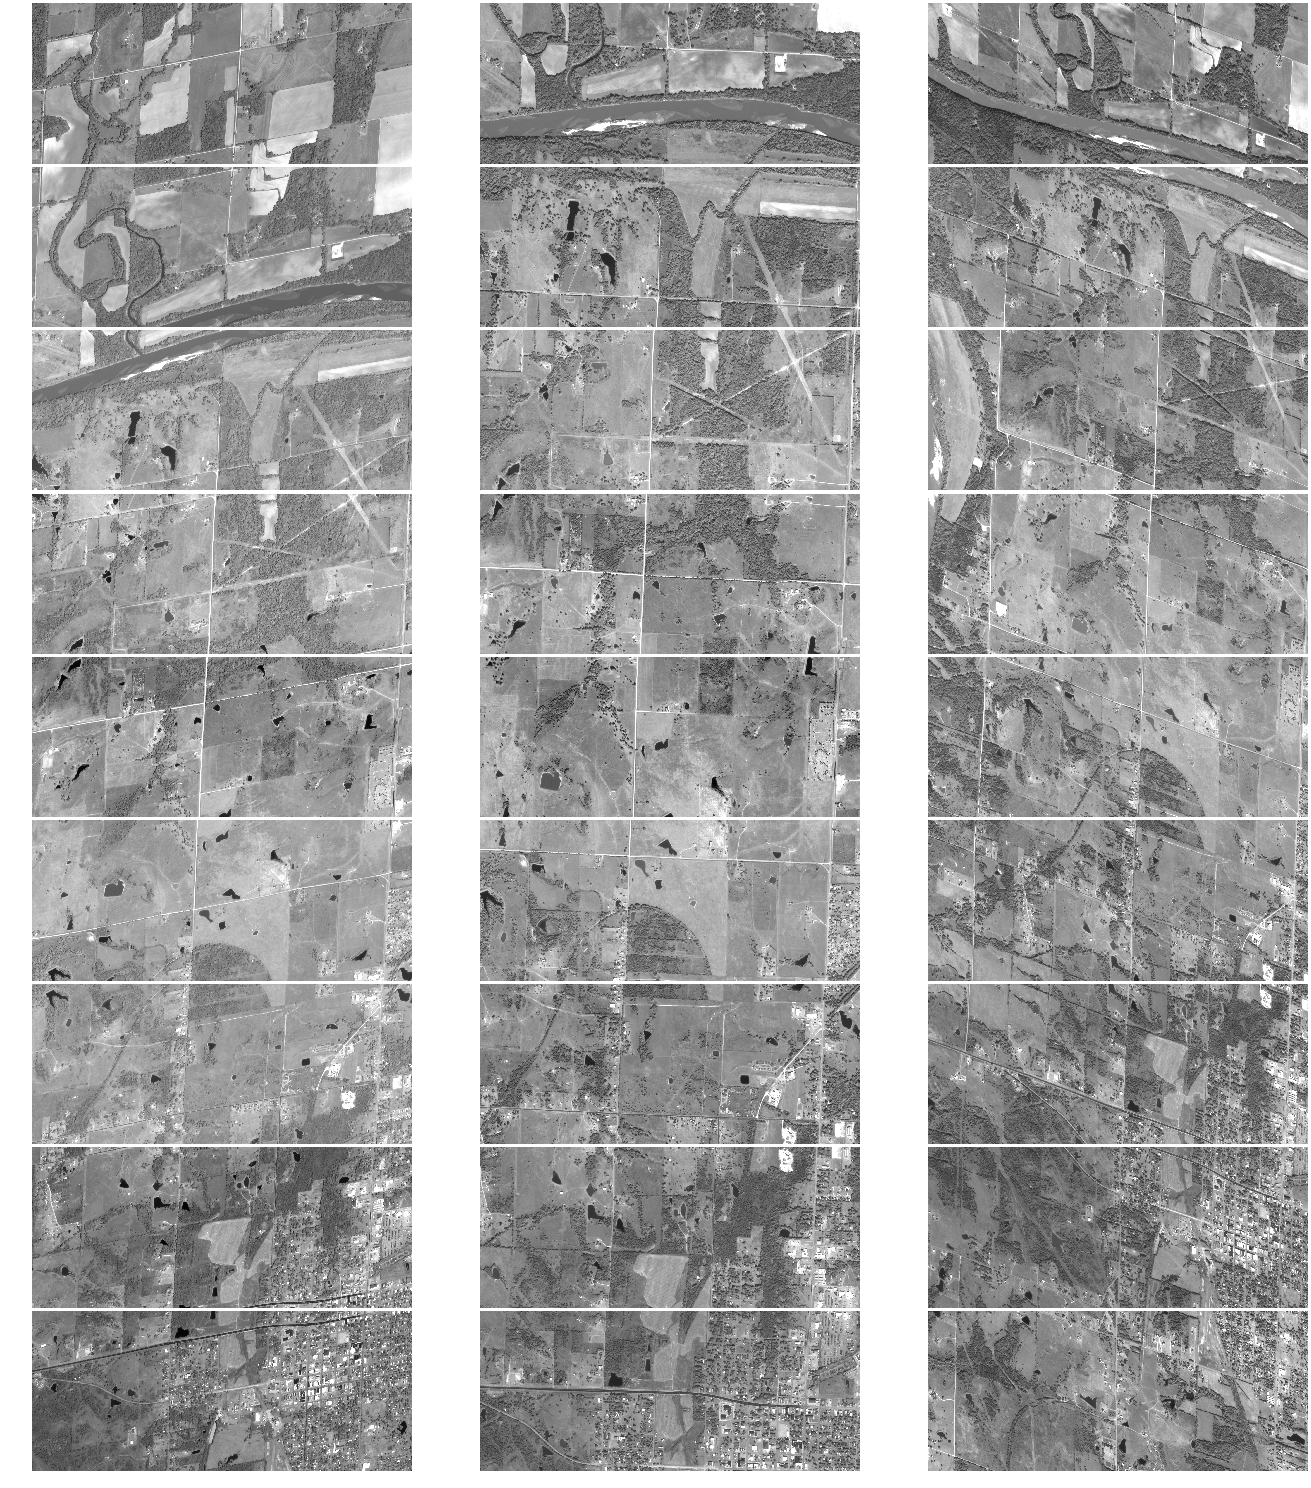
\includegraphics[width = 0.95\textwidth]{d3.png}
    \caption{Mosaic of d3. From left to right: 1Z, 7Z, 8Z}
    \label{}
\end{figure}



\section{Attitude of a Satellite}

\begin{figure}[h]
    \centering
    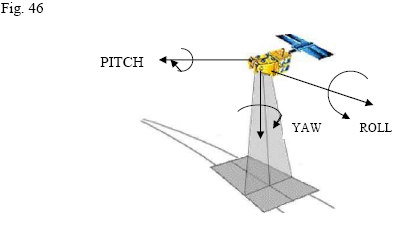
\includegraphics[width=0.5\textwidth]{figures/angles.jpg}
   \caption{ Roll, pitch and yaw angles.}
   \label{angles}
\end{figure}

\section{Satellite attitude error effects on stereo images}
\label{sec:sensibility}

\section{Correction of Relative Pointing Error}
\cite{de2014automatic}\\

A simple way to correct the relative pointing error is thus to transform one of the two images, in such a way that the corresponding points fall on the respective epipolar curves: given two images $u$, $v$ and a set of correspondences $(\textbf{x}_i , \textbf{x}'_i)_{i=1...N}$ , we search for a translation $f$ such that, for all $i$, the transformed point $f(\textbf{x}'_i)$ lies on the epipolar curve $epi^{\textbf{x}_i}_{u v}(R)$.
The desired transformation $f^{*}$ minimises the relative pointing error defined by:
\begin{align}
\label{minif}
f^* = \argmin{f} \dfrac{1}{N} \sum\limits_{i=1}^{N} d(f(\textbf{x}'_i), epi^{\textbf{x}_i}_{u v}(R))
\end{align}

From  \cite{de2014automatic}, we know that the epipolar curve $epi^{\textbf{x}_i}_{u v}(R)$ is approximated up to $0.05$ pixels by the straight line $F\textbf{x}_i$, where $F$ is
the affine fundamental matrix between the two views for the considered tile. As this fundamental matrix is an \textit{affine} fundamental matrix, all the lines $F\textbf{x}_i$ are parallel.

\subsection{Roll and Pitch Angles}
Because of sensitivity issues, we can take only roll and pitch error into account. Therefore according to section \ref{sec:sensibility}, we search for a transformation $f$ such that
\begin{align*}
f(\textbf{x}) = T\textbf{x}
\end{align*}
where $T$ is a translation:
\begin{align*}
T =
\begin{pmatrix}
1 & 0 & t_1 \\
0 & 1 & t_2 \\
0 & 0 & 1
\end{pmatrix}
\end{align*}
So we have, for $ \textbf{x} = (  x \; y \; 1)^T $,
\begin{align*}
f(\textbf{x}) = T\textbf{x} =
\begin{pmatrix}
x + t_1 \\
y + t_2 \\
1
\end{pmatrix}
\end{align*}

\subsubsection{Pointing error after rectification}
Without any additional restriction, we may assume that these lines are horizontal (otherwise just do a change of coordinates). The horizontal line $F\textbf{x}_i$ can be written, in homogeneous coordinates, as
\begin{align*}
F\textbf{x}_i = \left[ 0 \; 1 \; c_i \right]
\end{align*}
With these notations, for each point correspondence $(\textbf{x}_i , \textbf{x}'_i)$, we have
\begin{align*}
e(\textbf{x}_i, \textbf{x}'_i) = d(\textbf{x}'_i, epi^{\textbf{x}_i}_{u v}(R)) = d(\textbf{x}'_i, F\textbf{x}_i) = | y'_i + c_i|
\end{align*}

Here the error $e$ is invariant to any horizontal translation, thus the search for a translation minimizing the relative pointing error of formula (\ref{minif}) can be restricted to vertical translations only. With a vertical translation of parameter $t$, the error becomes
\begin{align*}
E(T) = \dfrac{1}{N} \sum\limits_{i=1}^{N} d(T\textbf{x}'_i, F\textbf{x}_i) = \dfrac{1}{N} \sum\limits_{i=1}^{N} | y'_i + t+ c_i|
\end{align*}
The translation that minimizes this sum is given by the geometric median (Weiszfeld, 1937) of the vector $(-y'_i - c_i )_{i=1...N}$.  The relative pointing error can thus be minimized in a tile by applying a translation to one of the images. Note that the median is robust against outliers, thus this correction procedure works well even in the presence of false matches.

\subsubsection{Pointing before after rectification}
In the general case, we have:
\begin{align*}
F\textbf{x}_i = \left( a_i \; b_i \; c_i \right)^T
\end{align*}
With these notations, the error to minimize is then:
\begin{align*}
E(T) &= \dfrac{1}{N} \sum\limits_{i=1}^{N} d(T\textbf{x}'_i, F\textbf{x}_i) = \dfrac{1}{N} \sum\limits_{i=1}^{N} \dfrac{|a_i(x'_i + t_1) + b_i(y'_i +t_2)+ c_i|}{\sqrt{a_i^2 + b_i^2}}
\end{align*}\\
As this fundamental matrix is an \textit{affine} fundamental matrix, all the lines $F\textbf{x}_i$ are parallel, \textit{i.e.}
\begin{align*}
F\textbf{x}_i = \left( a\; b\; c_i \right)^T
\end{align*}\\
We can then write the error as :
\begin{align*}
E(t_1, t_2) = \dfrac{1}{N\sqrt{a^2 + b^2}} \sum\limits_{i=1}^{N} |ax'_i+ by'_i + c_i + at_1 + bt_2|
\end{align*}
%$=\underset{y \in \mathbb{R}^n}{\operatorname{arg\,min}} \sum_{i=1}^N \left \| z_i-y \right \|_2$\\
%$y =
%\begin{pmatrix}
%- at_1 \\
%- bt_2 \\
%0
%\end{pmatrix}
%$
%$z_i =
%\begin{pmatrix}
%ax'_i \\
%by'_i \\
%c_i
%\end{pmatrix}$
\paragraph{Compute vectors $p$\\}
We can compute the vectors going from the projection of $\textbf{x}'_i$ on $F\textbf{x}_i$ to $\textbf{x}'_i$:
\begin{align*}
p(\textbf{x}_i, \textbf{x}'_i) &= d(\textbf{x}'_i, F\textbf{x}_i)\dfrac{1}{\sqrt{a_i^2 + b_i^2}}
\begin{pmatrix}
a_i \\
b_i
\end{pmatrix}  \\
&=
\dfrac{|a_ix'_i + b_iy'_i + c_i|}{a_i^2 + b_i^2}
\begin{pmatrix}
a_i \\
b_i \\
\end{pmatrix}
\end{align*}

And we have :

\begin{align*}
\begin{pmatrix}
t_1^* \\
t_2^* \\
\end{pmatrix} = -\text{median}\left[ p(\textbf{x}_i, \textbf{x}'_i)_{1 \leq i \leq N} \right]
\end{align*}



\subsection{Roll, Pitch and Yaw Angles}
If we assume that the scene is located at infinity with respect to the satellite, an error in the sensor attitude measurement can be modeled in image space as a translation composed with a rotation. Therefore we have
\begin{align*}
f(\textbf{x}) = RT\textbf{x}
\end{align*}
where $R$ is a rotation and $T$ a translation:\\
\begin{align*}
R =
\begin{pmatrix}
\cos(\theta) & -\sin(\theta) & 0 \\
\sin(\theta) & \cos(\theta) & 0 \\
0 & 0 & 1
\end{pmatrix}, \;
T =
\begin{pmatrix}
1 & 0 & t_x \\
0 & 1 & t_y \\
0 & 0 & 1
\end{pmatrix}
\end{align*}
So we have, for $ \textbf{x} = (  x \; y \; 1)^T $,
\begin{align*}
f(\textbf{x}) = RT\textbf{x} &=
\begin{pmatrix}
\cos(\theta) & -\sin(\theta) & t_x\cos(\theta) - t_y\sin(\theta)  \\
\sin(\theta) & \cos(\theta) & t_x\sin(\theta) + t_y\cos(\theta)  \\
0 & 0 & 1
\end{pmatrix} \textbf{x}  \\
&=
    \begin{pmatrix}
    \cos \theta (x + t_x) - \sin \theta (y + t_y)\\
    \sin \theta (x + t_x) + \cos \theta (y + t_y)\\
    1
    \end{pmatrix}
\end{align*}

When we take the yaw into accound, the error to minimize is :
\begin{align*}
E(R, T) &= \dfrac{1}{N} \sum\limits_{i=1}^{N} d(RT\textbf{x}'_i, F\textbf{x}_i) \\
&= \dfrac{1}{N} \sum\limits_{i=1}^{N} \dfrac{|a_i(x'_i + t_x)\cos \theta  - a_i (y'_i + t_y)\sin \theta  + b_i(x'_i + t_x)\sin \theta  + b_i  (y'_i + t_y)\cos \theta+ c_i|}{\sqrt{a_i^2 + b_i^2}}
\end{align*}\\

\subsection{After rectification}

Another way to correct the pointing error in the rectified setting is to find $R*$ and $T^*$ minimizing the pointing error defined as follow :
\begin{align}
    (R^*, T^*) = \argmin{R,T} \frac{1}{N} \sum_{i=1}^N d(TR\bm{x_i'}, F\bm{x}_i)^2
\end{align}
As in~\cite{de2014b}

After rectification, the horizontal line $F\bm{x}_i$ can be written, in homogeneous coordinates, as
\begin{align*}
F\bm{x}_i =  \begin{bmatrix} 0 & 1 & y_i \end{bmatrix}
\end{align*}
With these notations, if the model now includes a rotation $R$, for each point correspondence $(\bm{x}_i , \bm{x}'_i)$, we have
\begin{align*}
e(\textbf{x}_i, \textbf{x}'_i) = d(TR\bm{x}'_i, epi^{\textbf{x}_i}_{u v}(R)) = d(TR\bm{x}'_i, F\bm{x}_i) = |\sin \theta x_i'  + \cos \theta y_i' + t - y_i |
\end{align*}
where $\theta$ is the angle of the rotation.


Dans l'espace rectifié, on ne s'intéresse qu'à la deuxième coordonnées
$$
\min_{\theta, t}\sum_i |\sin \theta x_i'  + \cos \theta y_i' + t - y_i |
$$

Si on considère que l'angle de la rotation à appliquer est petit devant $2\pi$, il vient :
$$
\min_{\theta, t}\sum_i |\theta x_i'  + \theta y_i' + t - y_i |
$$
Cette approximation n'est pas dénué de sens étant donné la précision des instruments mesurant les angles sur Sentinel, Pleiages... ($50~\mu rad$) (sources à trouver). Donc même si Planet a des capteurs 100 fois moins précis, on reste en dessous du degré. Donc on s'attend à trouver un angle $\theta$ de moins d'un degré.

Que l'on peut exprimer matriciellement sous la forme de :
$$
\min_x \lVert Ax + b \rVert^2
$$

avec
$$
A =
\begin{pmatrix}
x_1' & 1 \\
x_2' & 1 \\
\vdots & \vdots \\
x_n' & 1 \\
\end{pmatrix}
$$

et
$$
x =
\begin{pmatrix}
\theta \\
t
\end{pmatrix}
$$

et

$$
b =
\begin{pmatrix}
y_1' - y_1\\
y_2' - y_2\\
\vdots\\
y_1' - y_1\\
\end{pmatrix}
$$
Convertir $\theta$ et $t$ dans l'espace original pour pouvoir les comparer


\appendix

Reminder: Matrix multiplication have always the origin as a fixed point. Common workaround using homogeneous coordinates.

\section{Rotations and translation}

In this part, we consider any point \((x, y) \in \mathbb{R}^2\). As translation and rotation do not commute, we will consider two cases: rotation followed by translation and translation followed by rotation, with \(R\) denoting the rotation of angle \(\theta\) and \(T\) denoting the translation of vector \((t_x, t_y)\). Naming \(f\) the resulting function.

\begin{align*}
    T &=
    \begin{pmatrix}
    1 & 0 & t_x \\
    0 & 1 & t_y \\
    0 & 0 & 1
    \end{pmatrix}
    \\
    R &=
    \begin{pmatrix}
    \cos \theta & -\sin \theta & 0 \\
    \sin \theta & \cos \theta & 0 \\
    0 & 0 & 1
    \end{pmatrix}
\end{align*}


\subsection{Rotation followed by a translation}
This happens when correcting the pointing error first with the rotation.

\begin{align*}
    f(\bm{x}) &= TR\bm{x} \\
    &=
    \begin{pmatrix}
    1 & 0 & t_x \\
    0 & 1 & t_y \\
    0 & 0 & 1
    \end{pmatrix}
    \cdot
    \begin{pmatrix}
    \cos \theta x - \sin \theta y \\
    \sin \theta x + \cos \theta y \\
    1
    \end{pmatrix}
    \\
    &=
    \begin{pmatrix}
    \cos \theta x - \sin \theta y + t_x\\
    \sin \theta x + \cos \theta y + t_y\\
    1
    \end{pmatrix}
\end{align*}

\subsection{Translation followed by a rotation}
This happens when correcting the pointing error first with the translation

\begin{align*}
    f(\bm{x}) &= RT\bm{x} \\
    &=
    \begin{pmatrix}
    \cos \theta & -\sin \theta & 0 \\
    \sin \theta & \cos \theta & 0 \\
    0 & 0 & 1
    \end{pmatrix}
    \cdot
    \begin{pmatrix}
    x + t_x \\
    y + t_y \\
    1
    \end{pmatrix} \\
    &=
    \begin{pmatrix}
    \cos \theta (x + t_x) - \sin \theta (y + t_y)\\
    \sin \theta (x + t_x) + \cos \theta (y + t_y)\\
    1
    \end{pmatrix}
\end{align*}


\bibliographystyle{plain}
\bibliography{biblio}
\end{document}

\end{document}
